\begin{figure}[htp]
	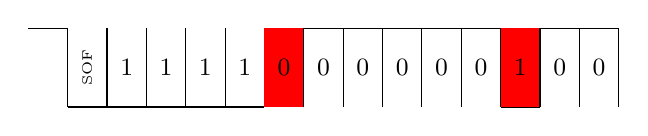
\begin{tikzpicture}[scale=1]
		\draw (0,1) -- ++(0.5,0);
		\foreach \x in {0.5,1,...,2.5}{
			\draw (\x,0) -- ++(0,1);
			\draw (\x,0) -- ++(0.5,0);
		}

		\node[rotate=90] at (0.75,0.5) {\tiny SOF};

		\foreach \x in {1,1.5,...,2.5}{
			\node[minimum height=1cm, minimum width=0.5cm] at (\x + 0.25,0.5) {\small 1};
		}

		%stuffing 1
		\draw (3,0) -- ++(0,1);
		\draw (3,1) -- ++(0.5,0);
		\node[fill=red, minimum height=1cm, minimum width=0.5cm] at (3.25,0.5) {\small 0};
		
		\foreach \x in {3.5,4,...,5.5}{
			\draw (\x,0) -- ++(0,1);
			\draw (\x,1) -- ++(0.5,0);
			\node[minimum height=1cm, minimum width=0.5cm] at (\x + 0.25,0.5) {\small 0};
		}
		
		%stuffing 2
		\draw (6,0) -- ++(0,1);
		\draw (6,0) -- ++(0.5,0);
		\node[fill=red, minimum height=1cm, minimum width=0.5cm] at (6.25,0.5) {\small 1};

		\foreach \x in {6.5,7}{
			\draw (\x,0) -- ++(0,1);
			\draw (\x,1) -- ++(0.5,0);
			\node[minimum height=1cm, minimum width=0.5cm] at (\x + 0.25,0.5) {\small 0};
		}
		\draw (7.5,0) -- ++(0,1);

	\end{tikzpicture}
	\caption{Bit Stuffing Example for 0x780 Identifier}
	\label{fig:can_stuffing}
\end{figure}